\documentclass{ximera}
\graphicspath{{./auto_generated_text/Week1CoordinateSystems/graphics/}{./graphics/}}
\title{Online Homework}
\begin{document}
\begin{abstract}
\end{abstract}
\maketitle

\begin{problem}
Find the Cartesian coordinates of the point $(\pi/2, \pi, 2)$, given in cylindrical coordinates.
\[
(x,y,z) = \answer{(0, -\pi/2, 2)}
\]
\end{problem}

\begin{problem}
Find the Cartesian coordinates of the point $(2, \pi, \pi/2)$, given in spherical coordinates.
\[
(x,y,z) = \answer{(-2,0,0)}
\]
\end{problem}

\begin{problem}
Find cylindrical coordinates for the point $\left(0, -1, 3\right)$, written in Cartesian coordinates. Your answer should satisfy $0\leq r$ and $0\leq \theta <2\pi$.
\[
(r, \theta, z) = \answer{(1, \pi, 3)}
\]
\end{problem}

\begin{problem}
Find spherical coordinates for the point $\left(-\sqrt{2}, \sqrt{2}, 2\sqrt{3}\right)$, written in Cartesian coordinates. Your answer should satisfy $0\leq \rho$, $0\leq \theta \leq 2\pi$, and $0\leq \phi \leq \phi$.
\[
(\rho, \theta, \phi) = \answer{(4, 3\pi/4, \pi/6)}
\]
\end{problem}

\begin{problem}
Consider the surface described in Cartesian coordinates by
\[
2z^2 = x^2 +y^2.
\]
Describe this surface with an equation in cylindrical coordinates, of the form $0=f(r,\theta, z)$.
\[
0=\answer{r^2-2z^2}
\]
FIGURE OUT HOW TO HANDLE THIS!!!
What type of shape is this?
\begin{multipleChoice}
\choice{Plane}
\choice{Cylinder}
\choice{Sphere}
\choice[correct]{Cone}
\choice{Other}
\end{multipleChoice}
\end{problem}

\begin{problem}
Consider the surface described in Cartesian coordinates by
\[
2z^2 = x^2 +y^2.
\]
Describe this surface with an equation in spherical coordinates, of the form $0=f(\rho, \theta, \phi)$.
\[
0=\answer{\rho^2\sin^2\phi - 2\cos^2\phi}
\]
FIGURE OUT HOW TO HANDLE THIS!!!
What type of shape is this?
\begin{multipleChoice}
\choice{Plane}
\choice{Cylinder}
\choice{Sphere}
\choice[correct]{Cone}
\choice{Other}
\end{multipleChoice}
\end{problem}

\begin{problem}
Consider the following region in $\mathbb{R}^3$.

\begin{image}
\begin{tikzpicture}
\node[inner sep=0pt] at (0,0)
    {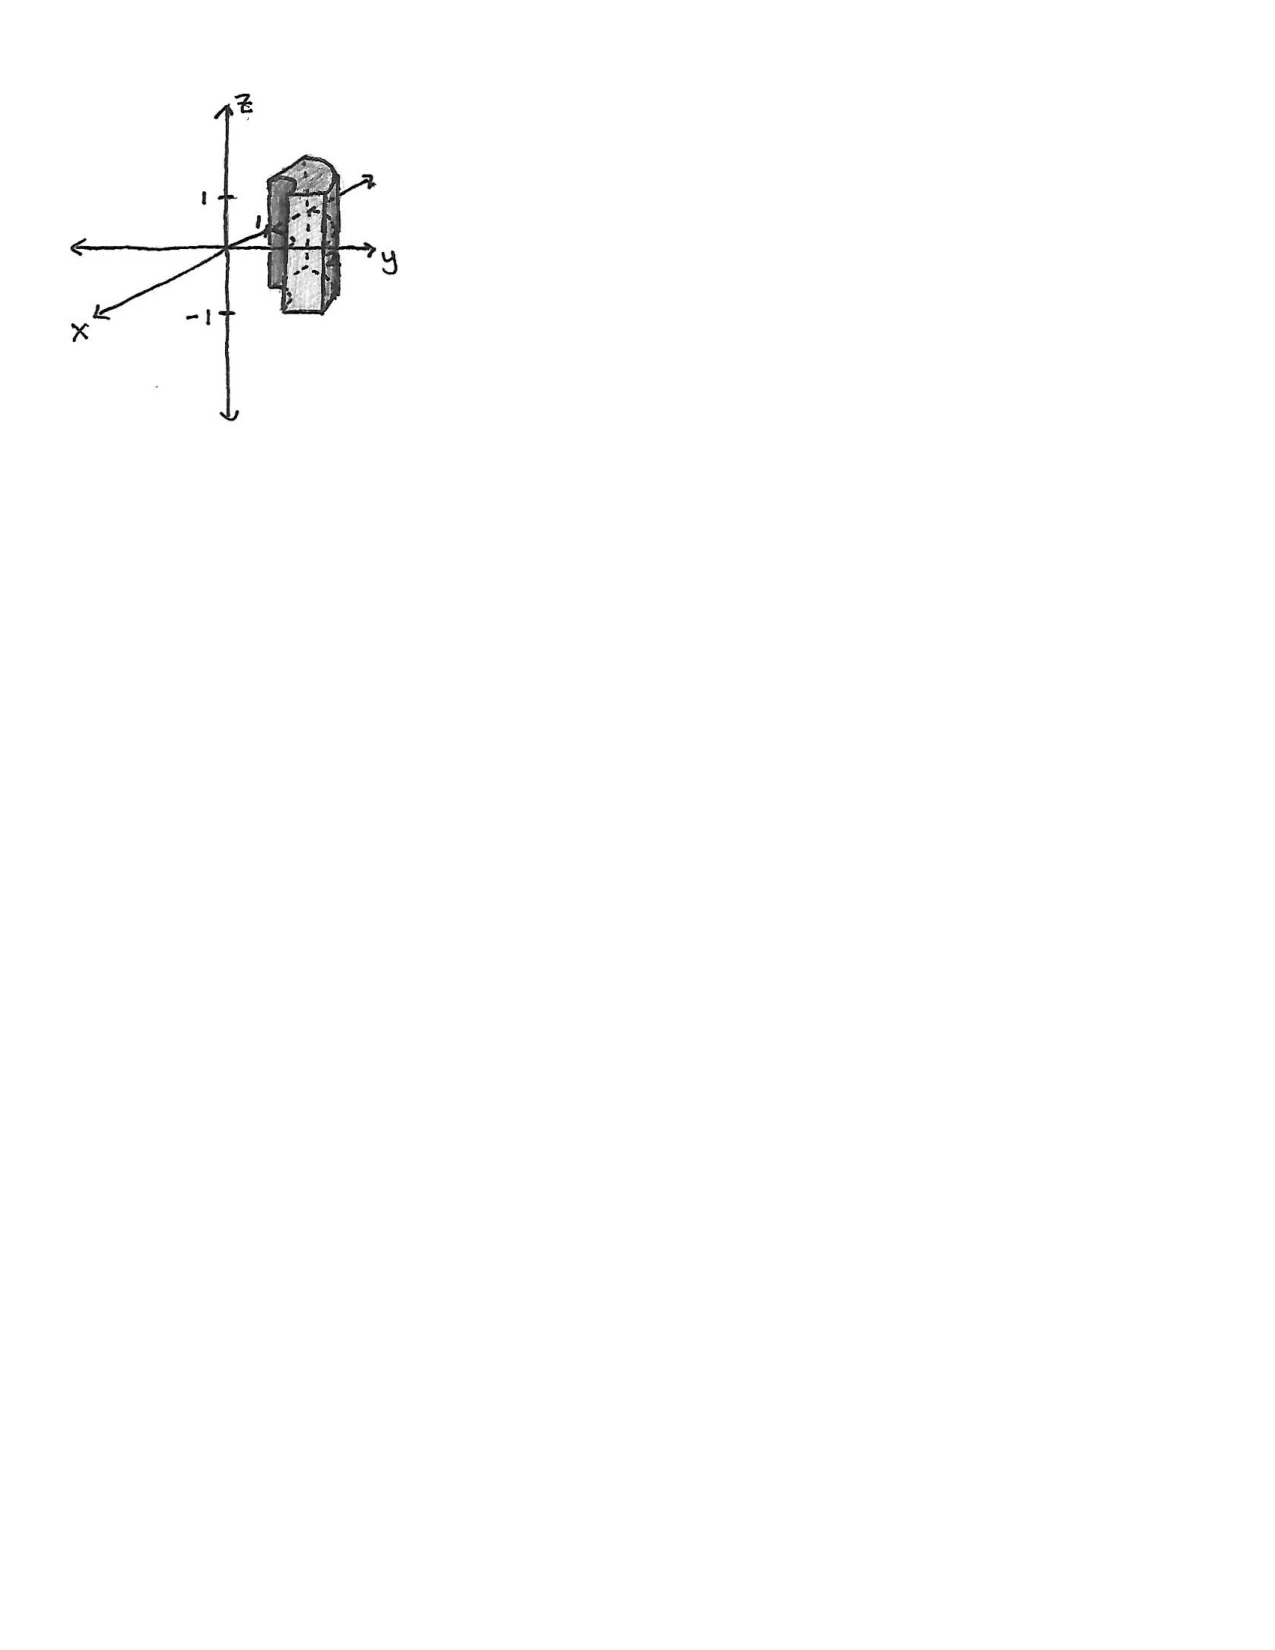
\includegraphics{cylinder_wedge}};
\end{tikzpicture}
\end{image}

This region is the set of points $(r, \theta, z)$, in cylindrical coordinates, satisfying the inequalities
\begin{align*}
&\answer{1}\leq r\leq \answer{2}\\
&\answer{\pi/2}\leq\theta\leq\answer{\pi}\\
&\answer{-1}\leq z\leq\answer{1}
\end{align*}

\end{problem}

\begin{problem}
Consider the following region in $\mathbb{R}^3$.

\begin{image}
\begin{tikzpicture}
\node[inner sep=0pt] at (0,0)
    {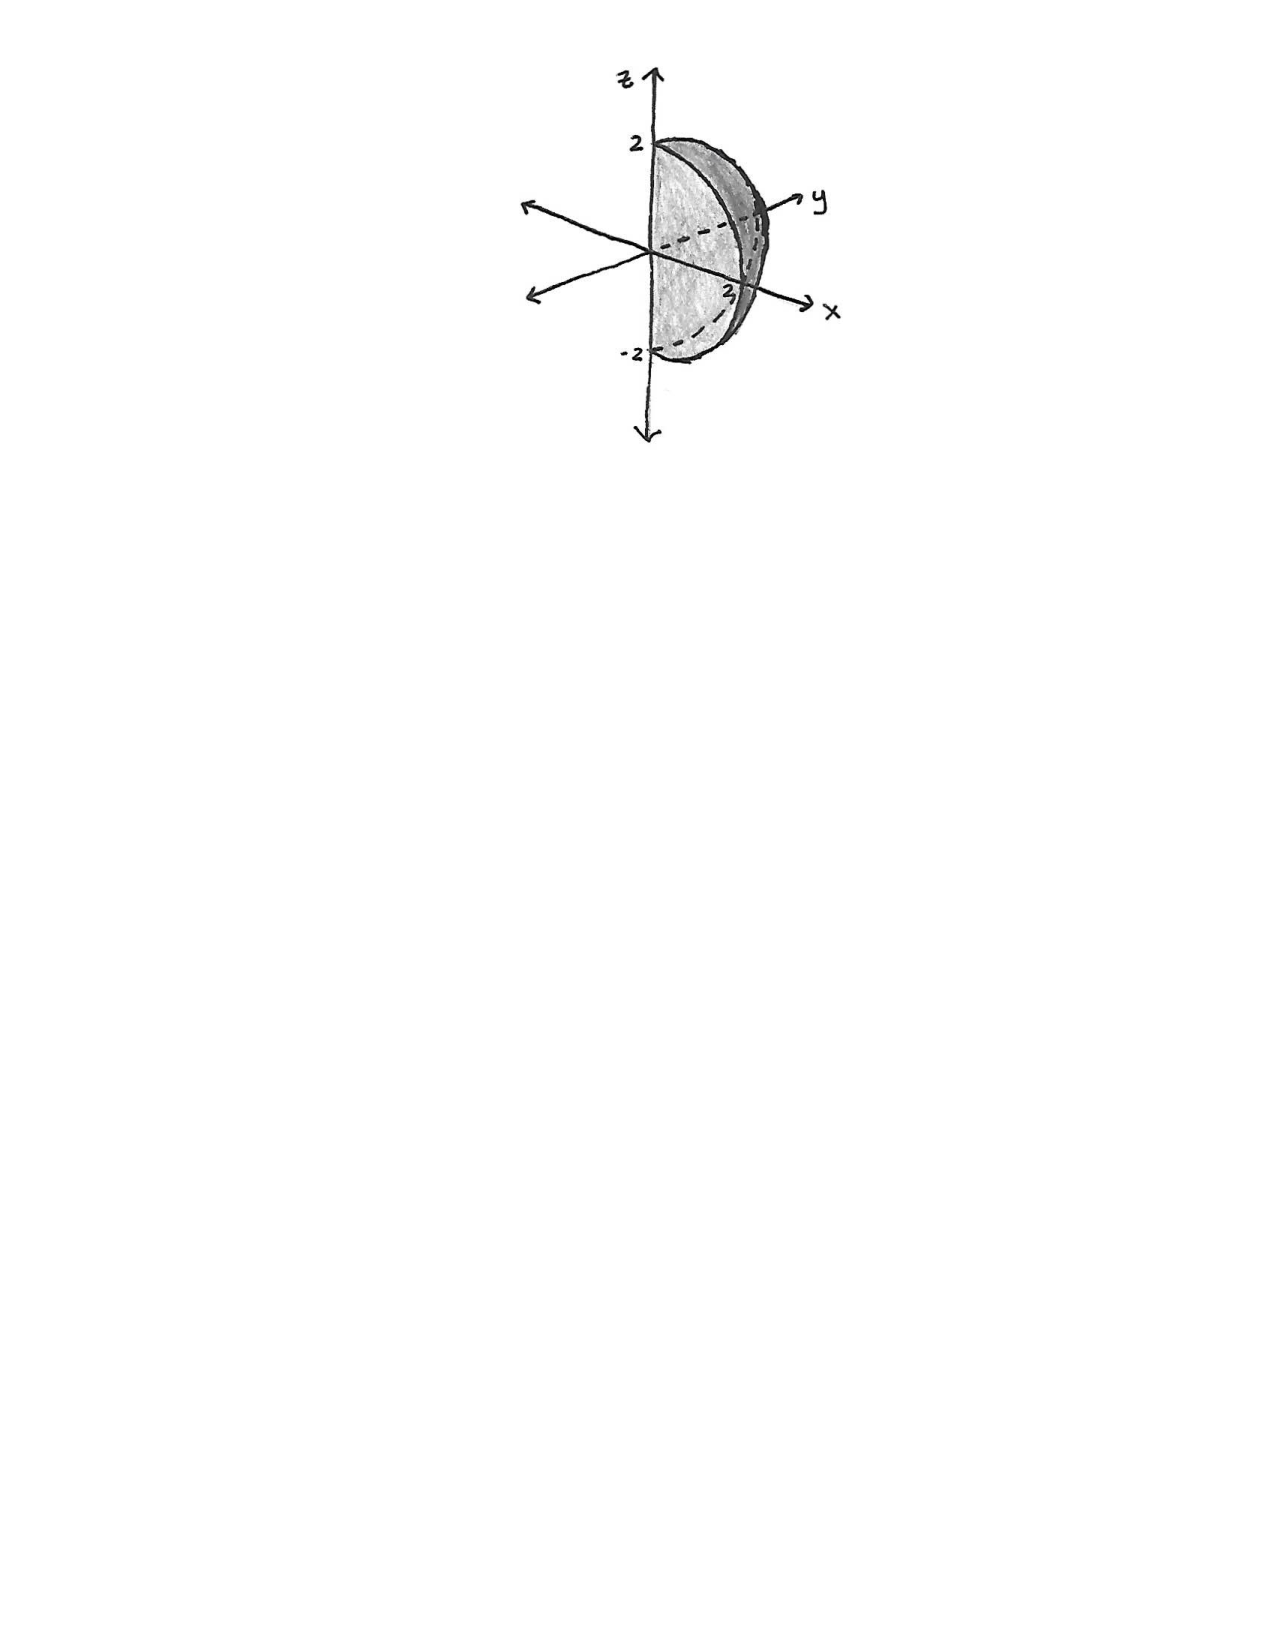
\includegraphics{sphere_wedge}};
\end{tikzpicture}
\end{image}

This region is the set of points $(\rho,\theta,\phi)$, in spherical coordinates, satisfying the inequalities
\begin{align*}
&\answer{0}\leq\rho\leq \answer{2}\\
&\answer{0}\leq\theta\leq\answer{pi/2}\\
&\answer{0}\leq\phi\leq\answer{pi}
\end{align*}

\end{problem}

\begin{problem}
For each of the following equations in cylindrical coordinates, select the type of shape they define.

FIGURE OUT CORRECT ANSWERS

$r = \cos\theta$
\begin{multipleChoice}
\choice{plane}
\choice{cylinder}
\choice{sphere}
\choice{other}
\end{multipleChoice}

$z = r\cos\theta$
\begin{multipleChoice}
\choice{plane}
\choice{cylinder}
\choice{sphere}
\choice{other}
\end{multipleChoice}

$z = -r$
\begin{multipleChoice}
\choice[correct]{plane}
\choice{cylinder}
\choice{sphere}
\choice{other}
\end{multipleChoice}
\end{problem}

\begin{problem}
For each of the following equations in spherical coordinates, select the type of shape they define.

FIGURE OUT CORRECT ANSWERS

$\rho = \cos\phi$
\begin{multipleChoice}
\choice{plane}
\choice{cylinder}
\choice{sphere}
\choice{other}
\end{multipleChoice}

$\rho = \sin\theta$
\begin{multipleChoice}
\choice{plane}
\choice{cylinder}
\choice{sphere}
\choice{other}
\end{multipleChoice}

$\rho\cos\theta\sin\phi = 1$
\begin{multipleChoice}
\choice[correct]{plane}
\choice{cylinder}
\choice{sphere}
\choice{other}
\end{multipleChoice}
\end{problem}

\end{document}